% Discussion notes: a topological analysis of the residual stream, as the next set of analyses after Exp 4 / 4b and
% the four attention-level topology analyses (exp4/LOG.md). Proposals only, no results.
% Build (from this folder): pdflatex residual_topology_notes.tex
\documentclass[10pt]{article}
\usepackage[letterpaper,hmargin=0.6in,vmargin=0.5in]{geometry}
\usepackage[T1]{fontenc}
\usepackage[scaled=0.92]{helvet}
\renewcommand{\familydefault}{\sfdefault}
\usepackage{microtype}
\usepackage{xcolor}
\usepackage{amsmath,amssymb}
\usepackage{enumitem}
\usepackage{tikz}
\usetikzlibrary{arrows.meta}
\usepackage[hidelinks]{hyperref}
% break the page before a block unless #1 of space is left (the needspace package isn't installed here)
\newcommand{\needspace}[1]{\par\vskip 0pt plus #1\penalty -200\vskip 0pt plus -#1}
\setlength{\parindent}{0pt}
\setlength{\parskip}{3pt}
\setlist{nosep,leftmargin=1.2em,itemsep=2pt}
\definecolor{cblue}{HTML}{2A78D6}
\definecolor{corange}{HTML}{EB6834}
\definecolor{cgreen}{HTML}{1BAF7A}
\definecolor{ink2}{HTML}{52514E}
\definecolor{muted}{HTML}{898781}
\definecolor{plane}{HTML}{F4F3EF}
\newcommand{\head}[1]{\par\vspace{5pt}{\large\bfseries #1}\\[-4pt]\rule{\linewidth}{0.5pt}\par}
\newcommand{\R}[2]{\par\needspace{9\baselineskip}\vspace{3pt}{\bfseries\color{cblue}#1}\ \textbf{#2}\par}  % keep a block's heading with its body
\newcommand{\row}[2]{\makebox[1.7cm][l]{\color{ink2}\small\itshape #1}\parbox[t]{\dimexpr\linewidth-1.7cm}{\small #2}\par}

\begin{document}

{\LARGE\bfseries From where heads look to what the stream carries}\\[2pt]
{\large Notes on a topological analysis of the residual stream}\\[2pt]
{\small\color{muted} Discussion notes for the next set of analyses. GPT-2 small. Builds on Exp 4 / 4b (a country at
position $\tau$; the final token $T$ is its capital, a wrong capital or a random token) and the four attention-level
topology analyses. Proposals, not results.}

\vspace{6pt}
\colorbox{plane}{\parbox{\dimexpr\linewidth-2\fboxsep}{\small
\textbf{The shift in one paragraph.} Everything so far measures \emph{attention}: how much a head at $T$ looks at the
country at $\tau$. Attention says where information could come from, not what is moved or kept. Each layer reads the
residual stream, and every head and MLP adds an update to it:
\[ x_{\ell+1}(T) \;=\; x_\ell(T) \;+\; \textstyle\sum_i h_{\ell,i}(T) \;+\; m_\ell(T). \]
The next analyses study these vectors directly: the head writes $h_{\ell,i}(T)$ (what each head moves) and the stream
states $x_\ell(T)$ (what is carried from layer to layer). They use the same paired design, nulls and independent checks
as before.}}

\vspace{6pt}
\begin{center}
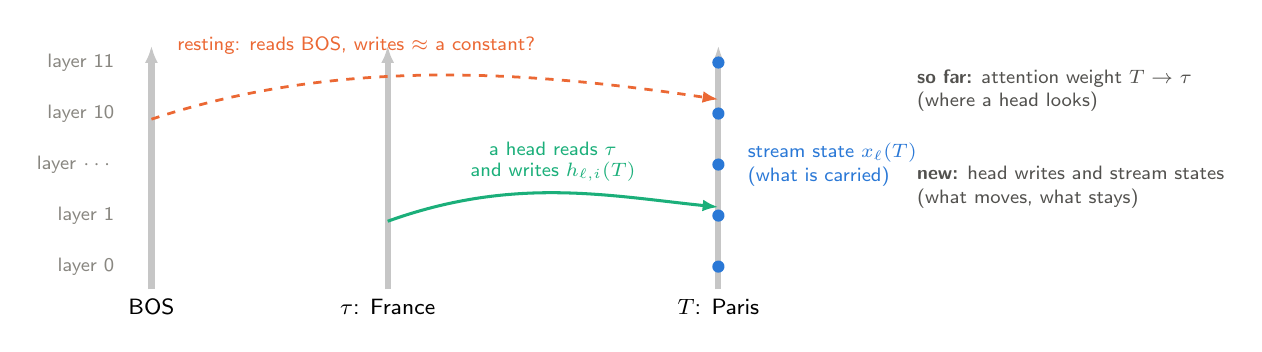
\begin{tikzpicture}[x=1cm,y=0.36cm,font=\footnotesize]
  \foreach \x/\lab in {0/{BOS}, 3/{$\tau$: France}, 7.2/{$T$: Paris}} {
    \draw[-{Latex[length=2.2mm]}, line width=2.2pt, gray!45] (\x,0) -- (\x,8.6);
    \node[below] at (\x,0) {\lab};
  }
  \foreach \y/\l in {0.8/0, 2.6/1, 4.4/$\cdots$, 6.2/10, 8.0/11} {\node[left, muted] at (-0.35,\y) {\scriptsize layer \l};}
  % a head at layer 1 reads the country and writes into T's stream
  \draw[-{Latex[length=2mm]}, cgreen, line width=1.1pt] (3,2.4) .. controls (4.6,4.0) and (5.8,3.3) .. (7.2,2.9);
  \node[cgreen, align=center] at (5.1,4.5) {\scriptsize a head reads $\tau$\\[-2pt]\scriptsize and writes $h_{\ell,i}(T)$};
  % a resting head reads BOS
  \draw[-{Latex[length=2mm]}, corange, dashed, line width=1pt] (0,6.0) .. controls (2.5,8.3) and (5.0,7.6) .. (7.2,6.7);
  \node[corange, align=center] at (2.6,8.6) {\scriptsize resting: reads BOS, writes $\approx$ a constant?};
  % stream states at T
  \foreach \y in {0.8,2.6,4.4,6.2,8.0} {\fill[cblue] (7.2,\y) circle (2.2pt);}
  \node[cblue, right, align=left] at (7.45,4.4) {\scriptsize stream state $x_\ell(T)$\\[-1pt]\scriptsize (what is carried)};
  % what we measured vs what is new
  \node[right, align=left, ink2] at (9.6,7.0) {\scriptsize \textbf{so far:} attention weight $T \to \tau$\\[-1pt]\scriptsize (where a head looks)};
  \node[right, align=left, ink2] at (9.6,3.6) {\scriptsize \textbf{new:} head writes and stream states\\[-1pt]\scriptsize (what moves, what stays)};
\end{tikzpicture}
\end{center}

\head{What we know that the residual analysis can test}
\begin{itemize}
\item Same-country heads in layers 0--4 (L0H2, L1H11, L3H0, L4H10) attend from the capital to its country at any
  distance. In layer 0, only the matching capital closes an attention loop.
\item The matching capital lowers late-layer resting on BOS at every distance ($-0.02$ to $-0.04$ against a wrong
  capital).
\item Previous-token heads look away from an adjacent same-country token. Head behaviour forms families but is ordered
  by depth only weakly.
\item \textbf{A structural fact that sets the scope.} Attention is causal, so the country's own stream at $\tau$ cannot
  see $T$. The match (``this is \emph{its} capital'') can only live in the stream at $T$. The $\tau$ stream can carry
  ``a country is here'', never ``and its capital follows''.
\item \textbf{A built-in null at layer 0.} $x_0(T)$ is just the capital's embedding plus its position. The own and
  wrong conditions use the same 11 capitals, so their layer-0 clouds are identical by construction. Any difference first
  appears after layer 0 writes.
\end{itemize}

\head{Proposed analyses}

\R{R1}{When does the stream at $T$ know the match?}
\row{object}{$x_\ell(T)$ for $\ell = 0..12$, its capital vs a wrong capital, on paired rows.}
\row{method}{Per layer: persistence of the pooled cloud, and bottleneck distance between the own and wrong clouds
against a label-permutation null. A linear probe is the non-topological baseline.}
\row{predict}{Identical at layer 0 (by construction), separable from layer 1 on, after L0H2's write.}
\row{counts if}{The topology shows something a probe does not. For example, own pairs form one tight component while
wrong pairs scatter by pair.}

\R{R2}{Do resting heads write nothing? (the no-op test)}
\row{object}{Each head's write $h_{\ell,i}(T)$ across sequences.}
\row{method}{For each head's write cloud: spread (total persistence, intrinsic dimension, norm), against the head's BOS
share, its capital vs a wrong capital.}
\row{predict}{Heads resting on BOS write a near-constant vector (a collapsed cloud). The late heads whose resting drops
under the matching capital expand.}
\row{counts if}{BOS share predicts collapse across heads, and the capital's BOS drop comes with expanded writes in the
same heads.}

\R{R3}{What does the stream carry about distance?}
\row{object}{The mean paired shift $m_\ell(\tau) = \mathbb{E}[x_\ell(T \mid \text{country at } \tau) - x_\ell(T \mid
\text{control})]$ for $\tau = 1..31$: a 31-point trajectory per layer.}
\row{method}{The trajectory's shape per layer: length, curvature, H0 scale, PCA dimension.}
\row{predict}{Early layers trace a distance-dependent curve; late layers collapse toward one point (``a country is
present''). This asks the advisor's local-vs-global question of the content rather than of attention, where we found
only a weak depth order.}

\R{R4}{How does information flow across layers?}
\row{object}{All states (sequence, layer) at $T$.}
\row{method}{Mapper with layer as the lens and average linkage (single linkage chained in the head analysis). Zigzag
persistence across consecutive layers, using the fact that the same sequences appear in every layer.}
\row{question}{Do the own and wrong branches split at some layer and stay split, or merge back (information
overwritten)?}

\R{R5}{Routes, not weights}
\row{object}{A layered graph on (layer, position). Edge weight = attention $\times$ the norm of the value vector
actually written (norm-based attention), not raw attention.}
\row{method}{Persistent homology of the flow graph from $\tau$ to $T$: count independent persistent routes, its capital
vs a wrong capital.}
\row{predict}{The layer-0 loop survives value weighting only if L0H2 writes a sizeable vector. Otherwise raw attention
overstated it.}

\R{+}{Causal companion: activation patching}
\row{}{Swap $x_\ell(T)$ between the own and wrong runs, layer by layer, and measure late BOS mass, the any-distance
heads' attention, and the capital's logit. Topology says where structure appears; patching says where it matters.}

\head{Extraction plan (one run, GPT-2 small, CPU)}
\begin{itemize}
\item TransformerLens hooks:
  \begin{itemize}
  \item \texttt{blocks.$\ell$.hook\_resid\_pre} plus \texttt{ln\_final}, for the stream states;
  \item \texttt{blocks.$\ell$.attn.hook\_result}, for the per-head writes (needs \texttt{model.set\_use\_attn\_result(True)});
  \item \texttt{blocks.$\ell$.hook\_mlp\_out}, for the MLP writes.
  \end{itemize}
  Store position $T$ only; keep $\tau$ and $\tau{+}1$ for the ``country present'' signal.
\item Same cached rows and 11 pairs. Conditions: control, own, wrong, random. $\tau \in \{31, 24, 16, 8, 1\}$ for the
  point clouds, and all 31 positions for the R3 means.
\item Size:
  \begin{itemize}
  \item stream states: 100 rows $\times$ 11 $\times$ 4 $\times$ 5 = 22{,}000 sequences $\times$ 13 layers, about
    0.45\,GB in fp16;
  \item head writes: a 30-row subset at 3 positions, about 0.9\,GB.
  \end{itemize}
  Minutes of compute; storage is the constraint.
\end{itemize}

\head{Pitfalls (lessons from the head analyses)}
\begin{itemize}
\item \textbf{Scale.} The residual norm grows with depth, and a few dimensions carry very large values (the
  attention-sink and massive-activation literature). Normalise per layer, centring and scaling as LayerNorm does, before
  any distance. Re-check with the top dimensions removed.
\item \textbf{Dimension.} 768 dimensions against a few thousand points: reduce with PCA to about 50, check stability at
  20 / 50 / 100, and bootstrap rows.
\item \textbf{Degenerate clouds.} The versions of a pair differ only at $\tau$ and $T$, so analyse paired differences,
  as with attention. Keep the caveat that the same 11 pairs mean consistent, not general.
\item \textbf{Chaining.} Rips H0 / single linkage made distinctive heads look isolated. Pair persistence with average
  linkage or kNN communities.
\item \textbf{Process.} Pre-register each R, and verify each one independently, as before.
\end{itemize}

\head{To decide together}
\begin{enumerate}[leftmargin=1.4em]
\item How do we define ``what the stream carries'': geometry (topology), decodability (probe), or causal effect
  (patching)? Proposal: all three, with topology leading and the other two as checks.
\item Which positions: $T$ only, where the match can live, plus $\tau$ and $\tau{+}1$ for the ``country present''
  signal?
\item What to start with: R2 (the no-op test, closest to the project's core claim) and R1, or R3 (the depth question)?
\item R5's weighting: norm-based (attention $\times$ $\lVert$value$\rVert$) or gradient-based attribution to the
  capital's logit?
\end{enumerate}

{\footnotesize\color{muted} Pointers:
\begin{itemize}
\item norm-based attention: Kobayashi et al., 2020;
\item attention rollout and flow: Abnar \& Zuidema, 2020;
\item attention sinks: Xiao et al., 2023; massive activations: Sun et al., 2024;
\item zigzag persistence: Carlsson \& de Silva, 2010;
\item intrinsic dimension across layers: Valeriani et al., 2023; TwoNN: Facco et al., 2017.
\end{itemize}
Our results: exp4/LOG.md, onepager/exp4b\_onepager.pdf, onepager/topology\_onepager.pdf.}
\end{document}
